% !TeX spellcheck = en_US

\chapter{Introduction}
\label{ch:intro}

\section{The Providentia++ Project}
\label{sec:providentia}

The Providentia Project~\cite{krammer2022providentia} aims to create a large-scale Intelligent Infrastructure System (IIS) that can provide autonomous vehicles and traditional vehicles with complementary information about each road user and the overall traffic situation.
By observing and detecting all road users from multiple perspectives, an IIS can greatly extend a vehicle's perception range, enabling it to plan its maneuvers more safely and proactively.
The primary goal of Providentia is to improve the safety and comfort of autonomous vehicles by reducing their reliance on on-board sensors and providing them with a better and spatially extended understanding of their surrounding scene.

There are several related projects in the field of IIS, including the Test Area Autonomous Driving Baden-Württemberg, the MEC-View project, and the local highway operator in Austria's road operator system~\cite{DBLP:journals/corr/abs-2112-05615}.
While these projects have similar goals, they are smaller in scale than Providentia and use different sensor types.
Additionally, many research contributions propose methods of making algorithmic use of the information provided by an IIS, or optimizing their function.

Providentia uses a combination of multimodal sensors, including radars, LIDARs, and cameras.
The radars and LIDARs provide distance measurements and can detect objects that are out of the camera's field of view.
The cameras capture a more distant environment than the LIDARs, but objects that are too far away appear small on the image and cannot be reliably detected.
The combination of these sensors provides redundant road coverage with overlapping field of views, accurate calibration, and robust detection and data fusion algorithms.

The RGB camera sensor captures visual information about the environment, which is used to generate the digital twin.
It can capture a more distant environment than the LIDARs but is prone to severe occlusions due to its low perspective.
The RGB camera sensor is essential for fusing multiple sensor perspectives and updating the digital twin, which includes information such as position, velocity, vehicle type, and a unique identifier for every observed vehicle.
By providing this digital twin to an autonomous driving research vehicle, Providentia demonstrates that it can be used to extend the limits of the vehicle’s perception far beyond its on-board sensors.
The update rate for the digital twin depends on the fusion-setup and the type of the used object detection network, and it can vary between 13.1Hz to 24.6Hz depending on the sensor setup.

% ----------------------------------------------------

\section{The A9 Testfield}
\label{sec:a9testfield}

\begin{figure}[htb]
    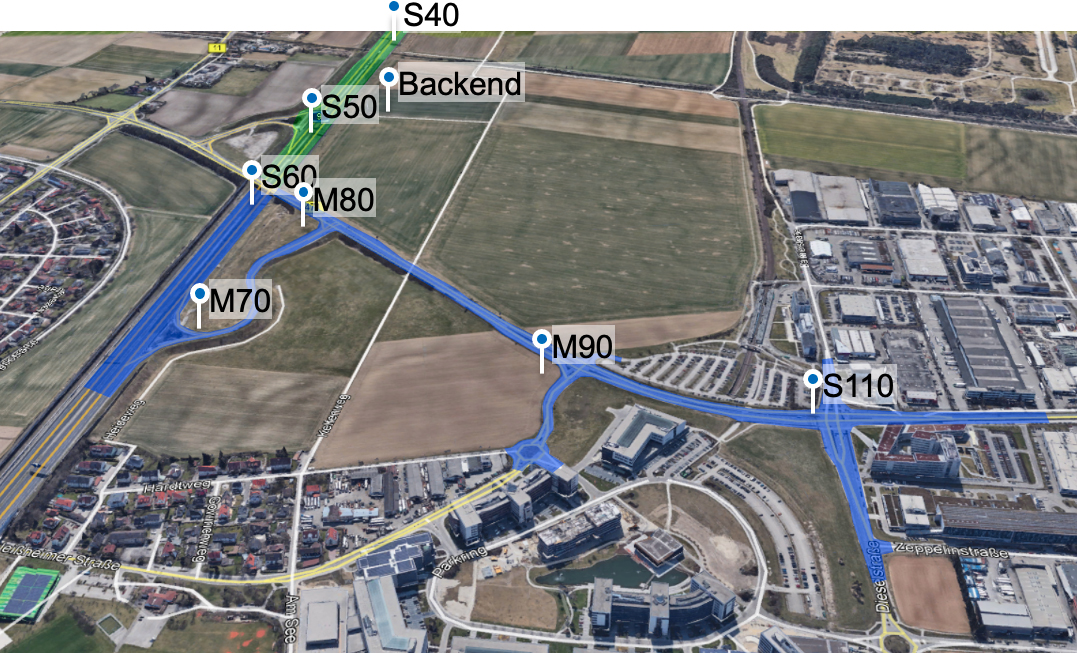
\includegraphics[width=\linewidth]{figures/teststrecke-gesamt}
    \caption{Overview of the Providentia A9 Test Stretch (Graphic produced using Google Maps).}
    \label{fig:providentia-test-area}
\end{figure}

At the heart of the Providentia Project is an expansive test area with multiple sensor stations.
The sensor stations are each equipped with RGB Camera, LIDAR and RADAR sensors.
These are used to test the sensor calibration-, road user detection-, sensor-fusion-, tracking-, and communication-solutions that are developed as part of the project.
An overview of the test area along the A9 highway near Garching Hochbrück, Germany is provided in Figure~\ref{fig:providentia-test-area}.

This work focuses on the RGB Camera sensors, which are installed at the designated stations.
The goal of this work is to develop a perception algorithm which can calculate a three-dimensional digital twin of any visible road user from the two-dimensional RGB camera input frames.
Previous work on the Monocular 3D Object Detection (\textit{Mono3D}) task in the scope of Providentia focused on solving this task for the sensor stations along the A9 highway~\cite{leonthesis}: \texttt{S40}, \texttt{S50} and \texttt{S60}.
In this work, we aim to generalize the Mono3D solution to cover the more urban sensor stations, in particular the cameras which are installed at the \texttt{S110} intersection.
This urban intersection setting is more challenging, because it does not allow for a fixed orientation of road users to be assumed by the monocular detector.
Instead, the detector must induce a contextual bias for each road user to determine their orientation angle.

Crucially, a high-definition (HD) map of the test area was also developed as part of the Providentia project using the OpenDRIVE format~\cite{dupuis2010opendrive}.
An overview of the map with a more detailed view of the S110 intersection is provided in Figure~\ref{fig:providentia-opendrive-map}.
Within this project, we aim to explore how the HD map of the test area can serve as  auxiliary sensory input to monocular detector.
We hypothesize, that the highly detailed map might provide the monocular detector with information about viable road user orientations.

For the demonstration purpose of this work, we focus our efforts on two cameras which are installed at the S110 sensor station: \texttt{S110-S1} and \texttt{S110-S2}.
Both cameras have a native resolution of 1920x1200 pixels and run at 60 Hz.
However, the \texttt{S110-S2} camera has a much longer detection range, as it is angled towards to horizon, whereas the \texttt{S110-S1} camera is focused downwards onto the intersection.

\begin{figure}[htb]
    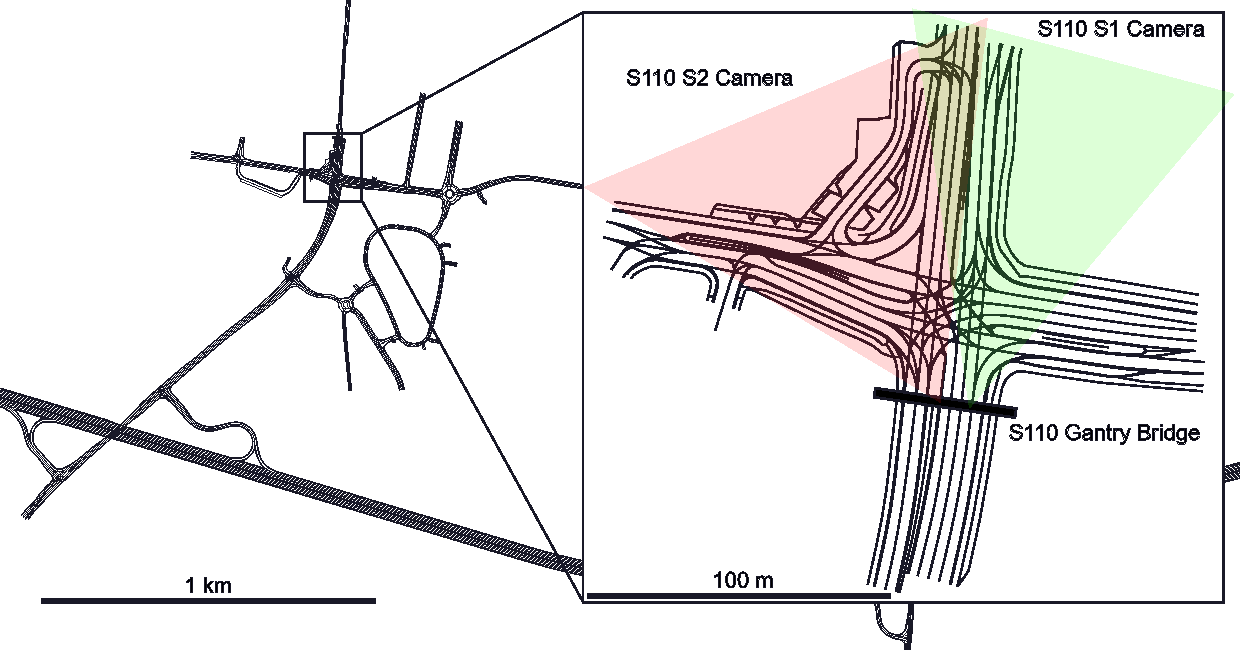
\includegraphics[width=\linewidth]{figures/map}
    \caption{Overview of the OpenDRIVE map of the Providentia test area, with zoomed in cut-out of the S110 intersection with its S1 and S2 cameras.}
    \label{fig:providentia-opendrive-map}
\end{figure}

% ----------------------------------------------------

\section{The A9R1 Dataset}
\label{sec:a9dataset}

In order to evaluate any object detection method, labeled data are required.
For this purpose, the \textit{A9R1} dataset was developed under the umbrella of Providentia.
The dataset annotates both LIDAR point-clouds with categorized 3D object bounding boxes, and RGB Camera frames with 2D cuboid labels.
Specifically, four scenes in the dataset provide the crucial combination of 3D LIDAR bounding box labels for 2D camera frames.
This labeling pair allows us to evaluate our monocular 3D object detector.
The four scenes in the dataset which do provide this required annotation mode are listed in table~\ref{tab:a9r1}.

\begin{table}[h]
    \centering
    \caption{A9R1 dataset scenes which provide camera frames annotated with 3D detection bounding boxes from LIDAR labels.}
    \label{tab:a9r1}
    \begin{tabular}{llllll}
        \toprule
        Scene & Perspective & \#Frames & \#Detections & Weather & Time of Day \\
        \midrule
        Scene 4 & S110 Camera S1 & 300 & 2918 & Sunny & Daytime \\
        Scene 4 & S110 Camera S2 & 300 & 2810 & Sunny & Daytime \\
        \midrule
        Scene 5 & S110 Camera S1 & 300 & 2958 & Sunny & Daytime \\
        Scene 5 & S110 Camera S2 & 300 & 2302 & Sunny & Daytime \\
        \midrule
        Scene 8 & S110 Camera S1 & 1200 & 8661 & Sunny & Daytime \\
        Scene 8 & S110 Camera S2 & 1200 & 11064 & Sunny & Daytime \\
        \midrule
        Scene 9 & S110 Camera S1 & 619 & 2327 & Rain & Night \\
        Scene 9 & S110 Camera S2 & 619 & 4668 & Rain & Night \\
        \bottomrule
    \end{tabular}
\end{table}

The dataset frame-rate is 10 Hz. The combination of 3D LIDAR Labels and RGB camera frames introduces an additional challenge in the form of synchronization delay \textemdash there may be up to 200 ms of difference between the 2D RGB frame and the 3D LIDAR annotation timestamps.
We will discuss this problem in more detail in Chapter~\ref{ch:evaluation}.
Each road user is also annotated with a category; one of \texttt{CAR}, \texttt{BUS}, \texttt{TRUCK}, \texttt{TRAILER}, \texttt{VAN}, \texttt{MOTORCYCLE}, \texttt{BICYCLE}, \texttt{PEDESTRIAN}, \texttt{EMERGENCY\_VEHICLE}, or \texttt{OTHER}.

% ----------------------------------------------------

\begin{figure}[htb]
    \includegraphics[width=\linewidth]{figures/mono3d}
    \caption{\textbf{On the left:} General dataflow in the Monocular 3D Object Detection task. For each instance of a recognized object in the RGB input frame, the detector must estimate a 3D pose parameter-set. The more variables the detector must estimate, the harder the task becomes. For example, elevation (i.e. the position z component) may be omitted. \textbf{On the right:} Figure 4.4 from~\cite{leonthesis}. Frame of a highway scene. In such a scenario, the detector may also omit the calculation of the heading (yaw) orientation angle and assume a fixed value.}
    \label{fig:mono3d-task-overview}
\end{figure}

\section{Monocular 3D Object Detection}
\label{sec:monodet}

\subsection{Estimands}
\label{subsec:estimands}

Monocular 3D Object Detection (\textit{Mono3D}) is the process of detecting three-dimensional objects from a single two-dimensional RGB camera output frame.
However, the term \textit{3D Object Detection} might be misleading in the context of this work.
In reality, the number of variables which a \enquote{3D} object detector may derive for an object far surpasses three, as can be seen in the following table~\ref{tab:mono3d-variables}.

\begin{table}[h]
    \centering
    \caption{Parameterization options for the output of a Monocular 3D Object Detector per object.}
    \label{tab:mono3d-variables}
    \begin{tabular}{lll}
        \toprule
        Variable & Description & Optional \\
        \midrule
        $X$/$Y$ & Position along the longitudinal/lateral axes.\ & \textbf{No} \\
        \midrule
        $L$/$W$ & Extent (length/width) along the longitudinal/lateral axes.\ & \textbf{No} \\
        \midrule
        $\delta X$/$\delta Y$/$\delta Z$ & Speed.\ Derivatives of the position/elevation variables.\ & \textbf{Yes} \\
        \midrule
        $Z$ & The elevation of the object over the road surface.\ & \textbf{Yes} \\
        \midrule
        $H$ & The height of the object.\ & \textbf{Yes} \\
        \midrule
        $\theta$ & Yaw (heading) angle, determines travel direction.\ & \textbf{No} \\
        \midrule
        $\phi/\gamma$ & Tilt/Roll angles, e.g.\ terrain slope or crash scenarios.\ & \textbf{Yes} \\
        \midrule
        $I$ & Identifier for the object across multiple frames.\ & \textbf{Yes} \\
        \midrule
        $C$ & Category of the object, e.g. \texttt{CAR} or \texttt{PEDESTRIAN}.\ & \textbf{No} \\
        \bottomrule
    \end{tabular}
\end{table}

We observe, that a minimal 3D Object Detector should actually estimate six dimensions per object: Birds-eye-view (BEV) positions $X$/$Y$, BEV size $L$/$W$, heading angle $\theta$ and category $C$.
Earlier work on the \textit{Mono3D} task for the Providentia project~\cite{leonthesis} focused on solving this task for the highway scenario.
On top of the minimum six variables, this early detector also calculated the object height.
However, as the early detector focused on the highway scenario, it was able to assume a fixed value for the $\theta$ variable.
This is illustrated on the right side of Figure~\ref{fig:mono3d-task-overview}.
As this work strives to generalize the \textit{Mono3D} solution beyond the highway, it must treat the $\theta$ value as non-fixed.
Interestingly, we facilitate this task by also estimating the identity $I$ variable, which then also allows us to estimate the planar speed $\delta X$/$\delta Y$ variables.
So we will end up with a 10-D detector in this work.

\subsection{Two-Stage Detection}
\label{subsec:twostage}

While many approaches are viable, the earlier Providentia \textit{Mono3D} detector by~\cite{leonthesis} used a so-called two-stage detection model.
As this work builds on top of~\cite{leonthesis}, we use the same approach.
Generally, the two-stage detector splits the detection task into two separate steps: a $2D$ instance segmentation step, and a $3D$ lifting step.
There are again many implementation options for these individual steps.
The steps are illustrated in Figure~\ref{fig:mono3d-two-stage}

\begin{figure}[htb]
    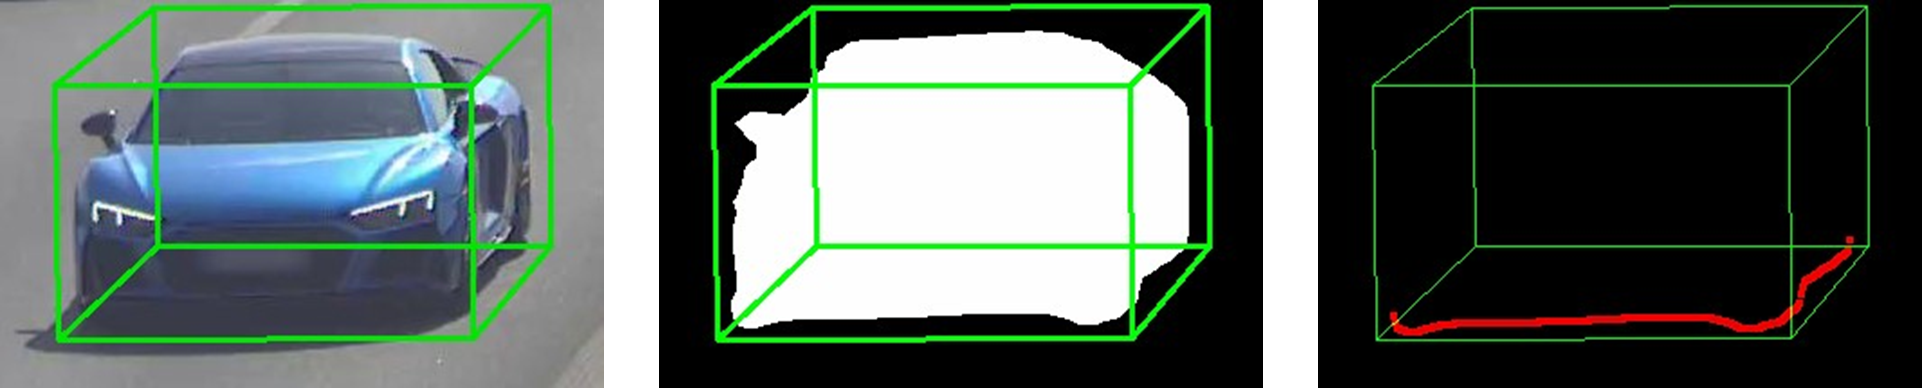
\includegraphics[width=\linewidth]{figures/two-stage-detection}
    \caption{Two-stage detection from camera image (left) via instance segmentation (middle) and $2D \rightarrow 3D$ lifting via the instance mask bottom contour (right). Graphic from~\cite{leonthesis}.}
    \label{fig:mono3d-two-stage}
\end{figure}

Within the taxonomy provided by~\cite{survey2022}, these are also called \textit{Result-based Lifting Methods}.
The primary advantage of this idea is that the 3D detector can benefit from highly polished, interchangeable, off-the-shelf instance segmentation models.
For example, the~\cite{leonthesis} detector exchanged \textit{Mask-RCNN}~\cite{he2017mask} in favor of \textit{Yolact-Edge}~\cite{liu2021yolactedge} in the first stage for performance reasons.
In this work we switch again, from \textit{Yolact-Edge} to \textit{YOLOv7}~\cite{wang2022yolov7} to improve the detection quality.
Another benefit is that stage two, the $2D \rightarrow 3D$ lifting stage, can be independently optimized, as the problem shifts from identifying the image areas occupied by relevant objects to estimating the three-dimensional properties of these objects.
The method proposed by~\cite{leonthesis} of lifting the $2D$ mask into $3D$ space via a $3D$ projection of the instance mask's bottom contour is applied and refined in this work.

The biggest hurdle towards a correct $3D$ vehicle pose estimation in an urban setting was identified by~\cite{leonthesis} as the $\theta$ (heading/orientation) value calculation.
The process by which an orientation angle can be estimated from the bottom contour is called \textit{L-Shape-Fitting}~\cite{zhang2017efficient}.
The vehicle bottom contour, which we want to use as an input to this calculation, can be quite noisy for many reasons, such as visual obstructions, upstream instance mask detection errors, or cropping at the image border (just to name a few).
Hence, an additional contextual bias is required for each object to correctly estimate its orientation angle.

\subsection{Use of Neural Networks}
\label{subsec:neural}

A Neural Network would most likely be a great choice for an algorithm to estimate not just the vehicle orientation $\theta$, but to perform the whole $2D \rightarrow 3D$ lifting stage.
For example, \textit{UrbanNet}~\cite{carrillo2021urbannet} implemented this approach with a Neural Network trained on synthetic data.
For this work, we are staying with a \enquote{rule-based}, non-neural approach for three reasons:

\begin{enumerate}
    \item Research continuity: The bottom-contour-based two-stage approach proposed by~\cite{leonthesis} is undoubtedly viable, there is no obvious reason to change the research direction.
    \item Explainability, Extendability, Maintainability: The \enquote{rule-based} approach allows for diagnosing and fixing particular failure modes.
    This is much harder with a neural network.
    \item Performance: A neural network estimator would most certainly require GPU resources to perform adequately in a real-time setting as required by the Providentia IIS. On the other hand, the non-neural approach can function purely on the CPU, leaving the sparse GPU resources to other tasks.
\end{enumerate}

For these reasons, this work explores exclusively non-neural \enquote{Software 1.0} \footnote{\hyperlink{https://karpathy.medium.com/software-2-0-a64152b37c35}{https://karpathy.medium.com/software-2-0-a64152b37c35}} solutions for the $2D \rightarrow 3D$ lifting stage.

\section{Relevance of HD Maps}
\label{sec:hdmap}

High-definition (HD) maps model the road network down to the detail of individual driving lane geometries.
In this work, we hypothesize that the HD-map can serve as a useful additional sensor to the \textit{Mono3D} detector.
In particular, we explore whether the HD map can serve as a viable source of vehicle orientation (heading) values.
In the first step, we developed a method to derive the likely heading value at a particular position on the road surface from the geometry of the enclosing lane boundaries.
This method is described with more detail in Chapter~\ref{sec:hdmapgrids}.
By converting the calculated $\overrightarrow{xyz}$ heading vectors at each position to $\text{RGB}$ colors, we are able to proof the general idea.
This is visualized in Figure~\ref{fig:headings-color-coded}.

\begin{figure}[htb]
    %\begin{tabular}{lll}
    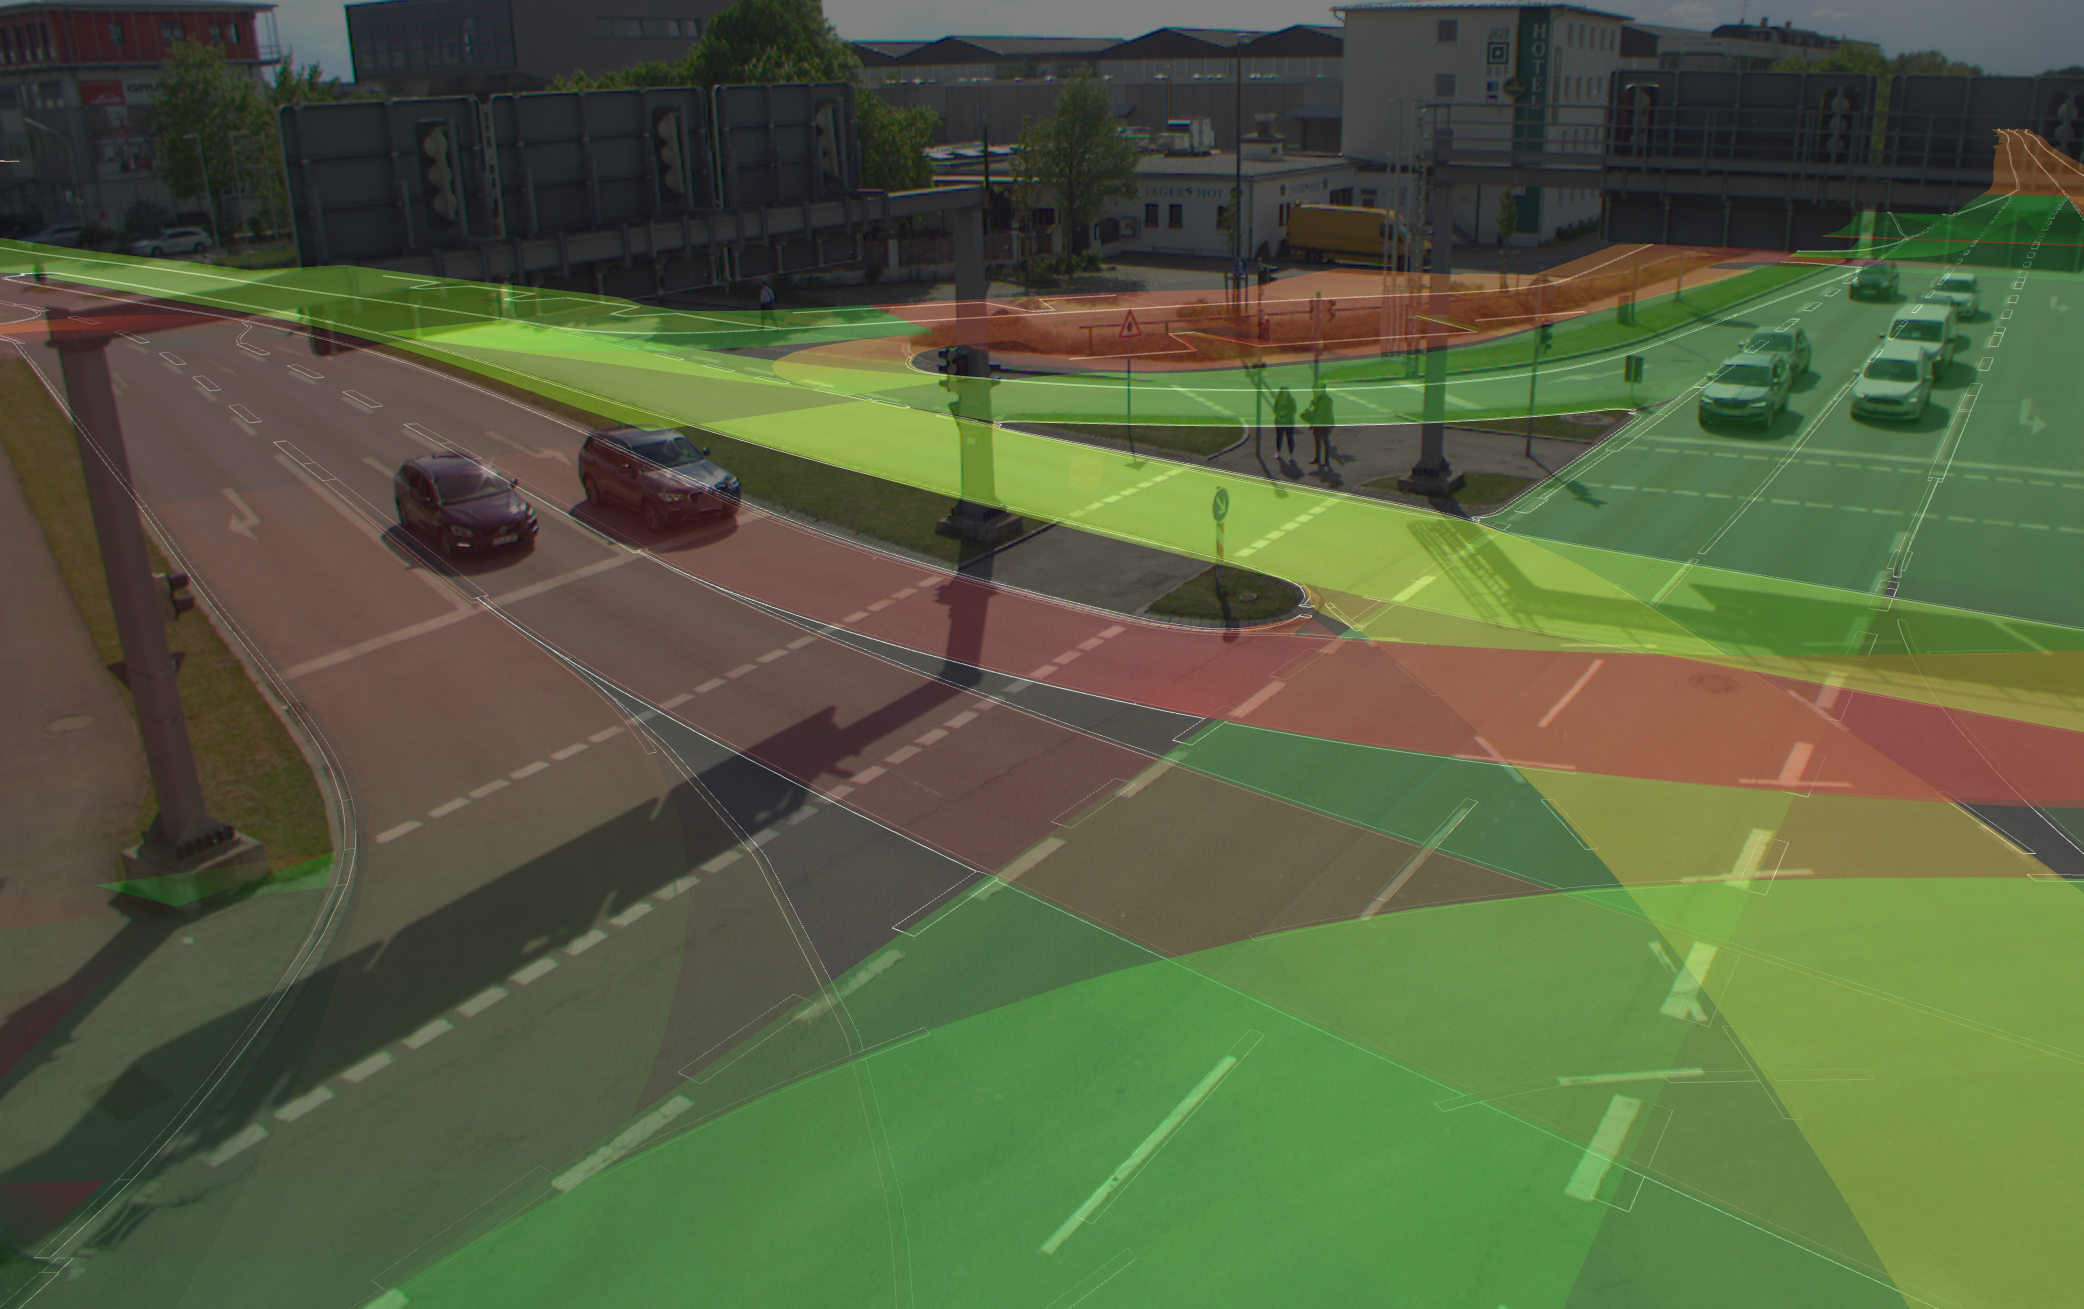
\includegraphics[width=0.4\linewidth]{figures/headings-colored-s2} % &
    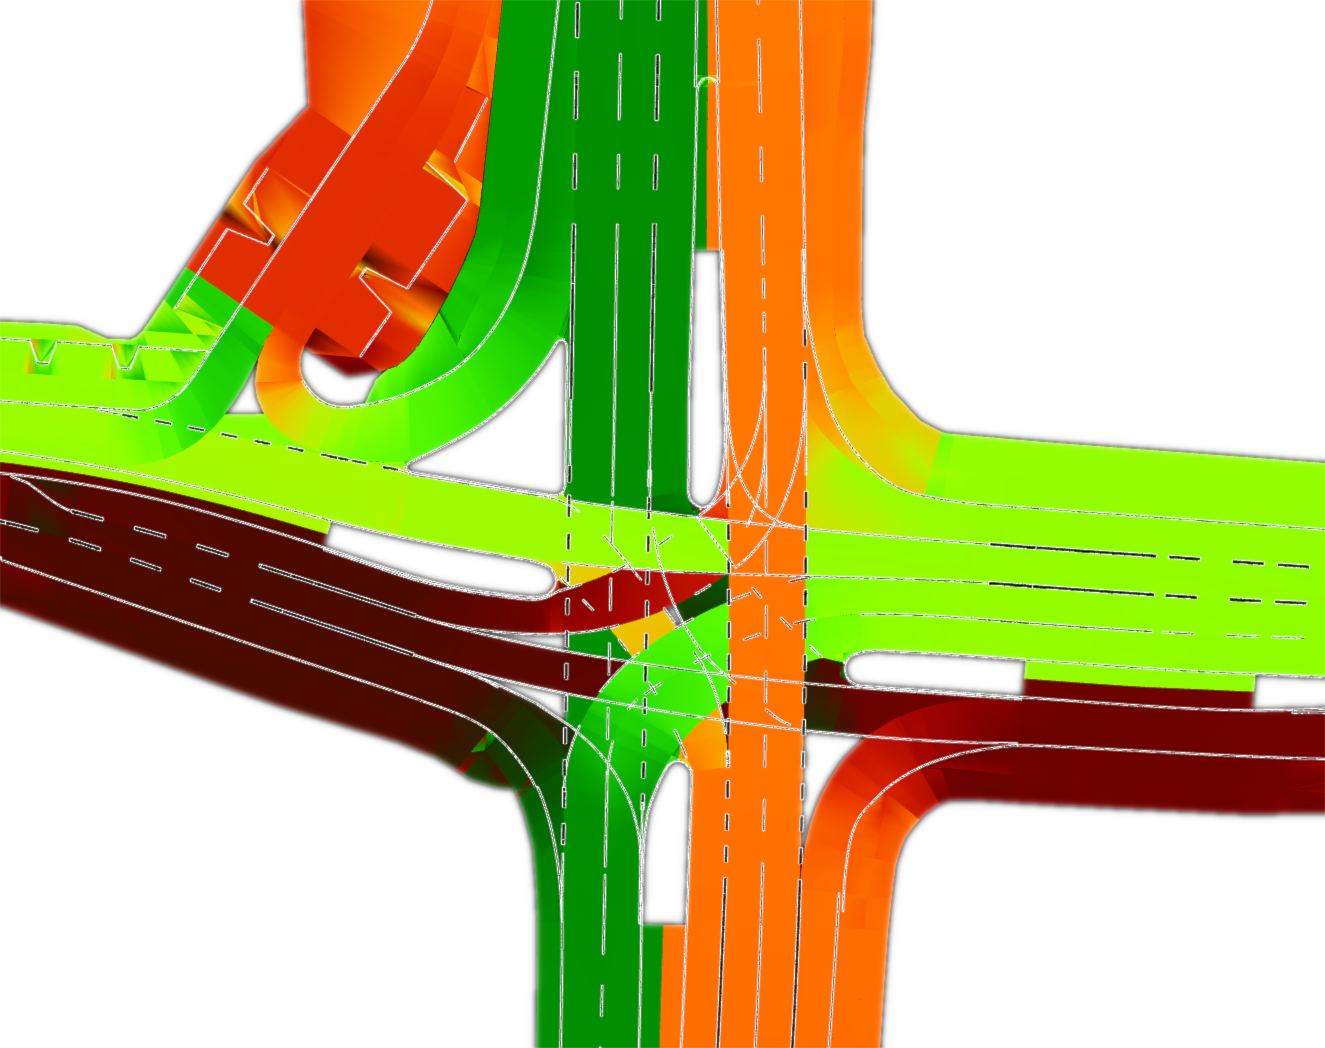
\includegraphics[width=0.29\linewidth]{figures/hdmap-heading-s110}
    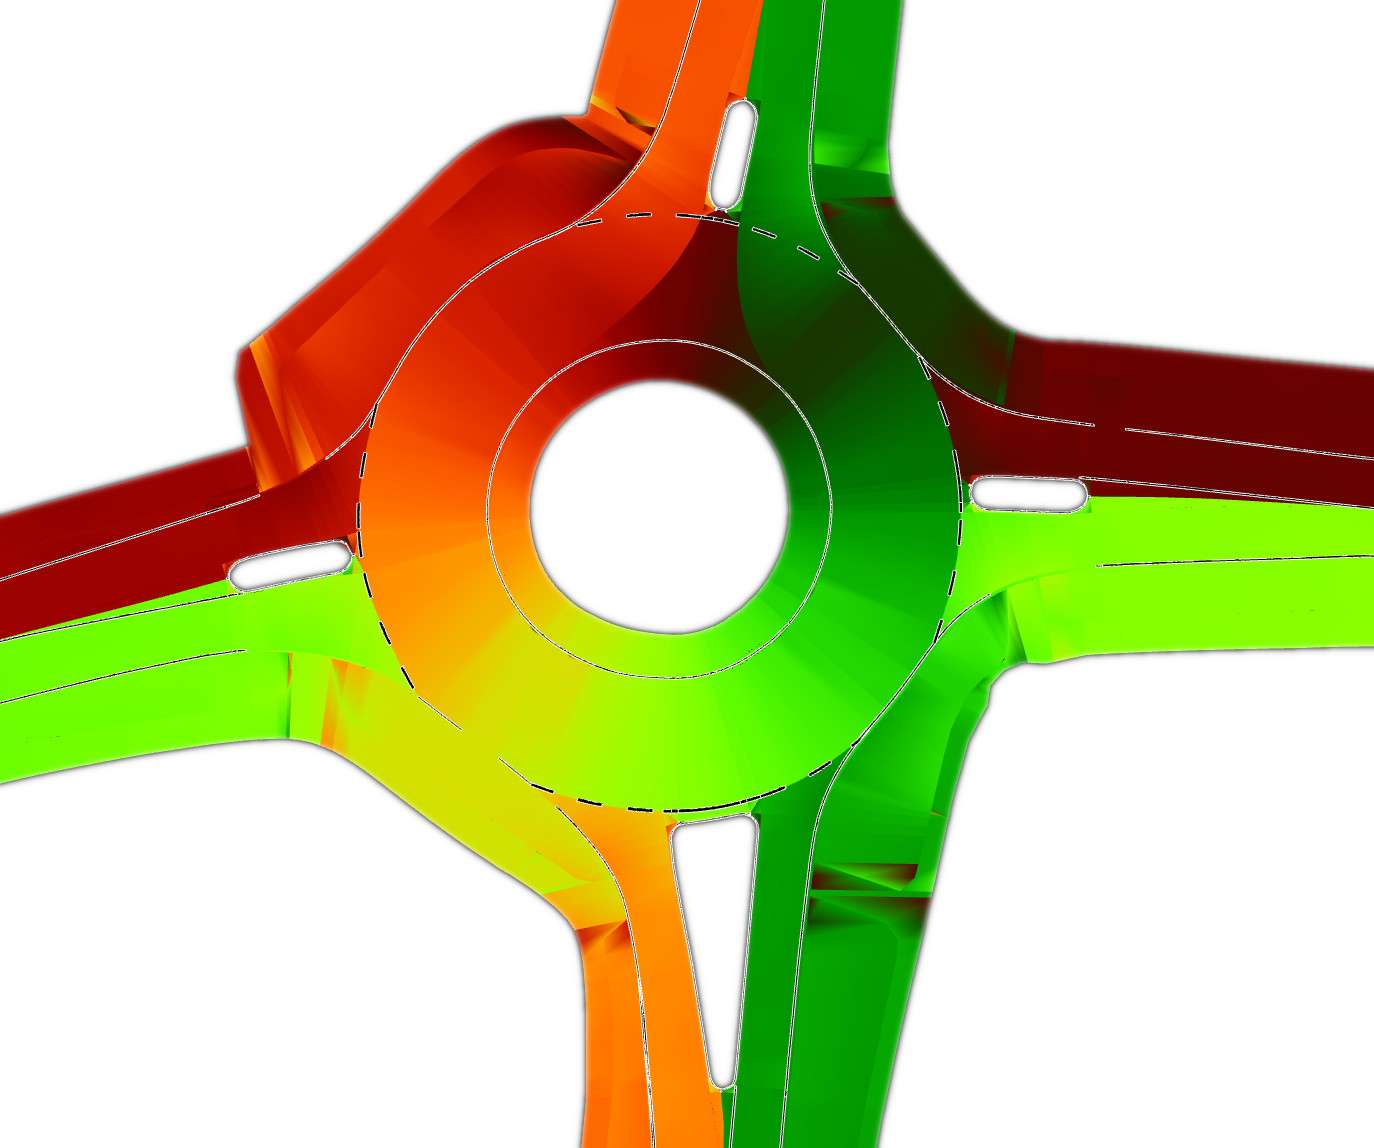
\includegraphics[width=0.29\linewidth]{figures/hdmap-heading-roundabout} % &
    %\end{tabular}
    \caption{Visualisation of heading vectors as RGB values, smoothly interpolated from the lane boundary geometry. \textbf{Left:} Colored heading overlays for the S110-S2 camera perspective. In the bottom-right corner, there are four overlapping lanes. \textbf{Middle:} RGB heading visualization for the whole S110 intersection. \textbf{Right:} RGB heading visualization for a roundabout.}
    \label{fig:headings-color-coded}
\end{figure}

From this proof-of-concept visualization of the heading vectors, it becomes apparent that the map-derived headings may serve well as an additional per-pixel feature for the \textit{Mono3D} detector.
But it also becomes apparent, that there may always be many possible overlapping heading options provided by the HD map, as there may always be many overlapping lanes \textemdash especially in the context of urban intersection scenarios.
The left-most image of Figure~\ref{fig:headings-color-coded} illustrates this problem quite well.
Here we see color-coded headings overlaid on top of a frame from the \texttt{S110-S2} camera.
Towards the bottom-right corner of the image, there are locations with up to four overlapping lanes, which provide four distinct heading options!
Therefore, an additional information source is needed to resolve ambiguities among multiple heading options.

% ----------------------------------------------------

\section{Tracking Enters the Picture}
\label{sec:tracking}

\subsection{Screen-Space Tracking}
\label{subsec:sstracking}

In face of the aforementioned uncertainties when deciding between ambiguous heading options, it might be useful to consider previously known spatial orientations of a vehicle.
Consider a scene such as the one shown in Figure~\ref{fig:tracking}.

\begin{figure}[htb]
    \centering
    \includegraphics[width=0.7\linewidth]{figures/tracking}
    \caption{Visualisation of a \textit{Mono3D} detection scenario where tracking resolves a heading ambiguity.}
    \label{fig:tracking}
\end{figure}

In this scene, the \textit{Mono3D} detector $C$ observes the instance mask of vehicle $M$.
Through the screen-space bounding box of $M$, the detector is able to associate this instance mask with detections from previous frames \textemdash $P_0$ and $P_1$.
The mask $M$ also allows for the calculation of the 3D position $P_2$.
The detector then performs a lookup for $\theta$ (heading) options at location $P_2$, and obtains two possible headings: $\theta_1$ and $\theta_2$.
As the detector must now pick one of these heading options, it may use the given knowledge of previous historical positions ($P_0$ and $P_1$) for $M$ to bias towards $\theta_1$ as the more likely orientation.
This is, because the detector assumes that vehicles move in a continuous direction more often than not, and erratic turns are less likely than forward motion.

To express this intuition formally, given a detection $M$ at time $t$ which is associated with a set of historical positions $P=\{p_{t},\mathellipsis,p_{t-T}\}$, we wish to pick $\theta(M)$ such that \[\sum_{\delta=1}^{\delta=T} |\theta(M) - \text{atan2}(p_t - p_{t-\delta})|\] is minimal.
In this work, the storage and retrieval of historical positions for the screen-space bounding box of a detection is accomplished using the \textit{SORT}~\cite{bewley2016simple} object tracking algorithm.

\subsection{Birds-Eye-View Tracking}
\label{subsec:bevtracking}

We use screen-space tracking to aid in the ranking of heading options.
However, the same tracking algorithm can also be used at a later stage for a different pupose:
In Birds-Eye-View \textit{(BEV)} tracking, objects are tracked in $3D$ space on the $X$/$Y$ axes rather than in camera image space.
This is where the \textit{Kalman-Filters}~\cite{welch1995kalman} which are at the heart of the \textit{SORT}~tracking algorithm really develop their potential as denoisers of physical measurements.
Fully implemented, they could denoise every variable of a tracked detection.
However, in this work, we will only use them to stabilize position and speed estimates.

\section{Inherent Functional Limitations}
\label{sec:limits}

As the origins, goals and methods of this work are now introduced, we can already identify functional limitations which are going to be inherent to our approach.
These limitations must be tackled by future work (see Chapter~\ref{ch:future}).

\begin{enumerate}
    \item \textbf{Bad detection quality for road users with highly cropped or obstructed instance masks}: Both the bottom-contour based L-Shape-Fitting algorithm, and the estimation of the vehicle position from the instance mask require an unobstructed full view of the road user to function optimally.\ Any obstruction of the view will degrade the estimation quality.\ Such an obstruction may be a stationary object in front of the road user, another road user, a weather condition like snow/rain/fog, or simply the field-of-view \textit{(FOV)} limit of the sensor.
    \item \textbf{Bad detection quality for road users in legal or physical peril:} Our \textit{Mono3D} detection approach assumes that road users do not fly, do not lie on their side, do not move sideways, and are always aligned with a legal traffic flow direction as parsed from the HD-map.\ Therefore, the 3D pose estimation for any road user which violates one of these assumptions will be as bad as the the day this road user is probably experiencing.
\end{enumerate}

\section{Research Objective}
\label{sec:objective}

In summary, the research objective for this work is to address the truthfulness of the following hypothesis: \textit{A two-stage \textit{Mono3D} detector with an instance-mask bottom-contour based estimator in the second stage can function well within an urban intersection setting, if the estimator is assisted by additional information from an HD map}.

\section{Contributions}
\label{sec:contributions}

This work presents the following research contributions:

\begin{enumerate}
    \item An Augmented L-Shape-Fitting Algorithm which supports tracking and HD-Map confidence inputs.
    \item A lookup strategy for vehicle bottom contours within the HD Map to derive Yaw Options with associated confidence values.
    \item An HD-Map Rasterization Algorithm to support fast bulk lookup of heading options for a vehicle bottom contour.
    \item A formula to derive the plausibility of a yaw hypothesis for a detected vehicle from a series of historical positions for the same vehicle.
    \item An algorithm to calculate the physical position and height of a vehicle, given its instance mask height and physical width/length.
    \item An algorithm to calculate 3D bounding boxes for Vulnerable Road Users (Pedestrians and Bicycles) from their Instance Mask Bottom Contour.
\end{enumerate}
